\subsection*{Q. 4}
\begin{longtable}[c]{llllll}
         &          &          & $A_2$    & $A_1$    & $A_0$    \\
\endfirsthead
%
\endhead
%
$\times$ &          &          & $B_2$    & $B_1$    & $B_0$    \\ \hline
         &          &          & $A_2B_0$ & $A_1B_0$ & $A_0B_0$ \\
         &          & $A_2B_1$ & $A_1B_1$ & $A_0B_1$ &          \\
         & $A_2B_2$ & $A_1B_2$ & $A_0B_2$ &          &          \\ \hline
$C_5$\quad & $C_4$    & $C_3$    & $C_2$    & $C_1$    & $C_0$   
\end{longtable}
\par Starting with the traditional vertical multiplication, we found out that: \ding{172} a 3-bit multiplication is made up of three partial products; \ding{173} each partial product, is a 1-bit $\times$ 3-bit, while bits can only be 0 or 1, this multiplication doesn't have carry out, and thus can simply use three; \emph{and gate} to denote them \ding{174} the partial products are added up to give the final result. Formally, we say:
\begin{align*}
C_0&=A_0B_0&\text{(no carry out)}\\
\{\text{Carry}_1, C_1\}&=A_1B_0+A_0B_1&\text{LHS = 2 $\times$ Carry$_1$ + $C_1$}\\
\{\text{Carry}_2, C_2\}&=A_2B_0+A_1B_1+A_0B_2+\text{Carry}_1\\
\cdots\\
\{\text{Carry}_4, C_4\}&=A_2B_2+\text{Carry}_3\\
C_5&=\text{Carry}_4
\end{align*}
\par A.k.a., since multiply takes \emph{AND} operation of the all binary combination from the bits of A and B and add the result with shifting \emph{i+j (i,j denotes the indices of bits in A and B)} operations. To express the final result in binary form, we only take the least bit of output sum and feed the rest bits of output sum together with the carry out bit into the augend input of the next full adder. \\
\vspace{1em}
\centerline{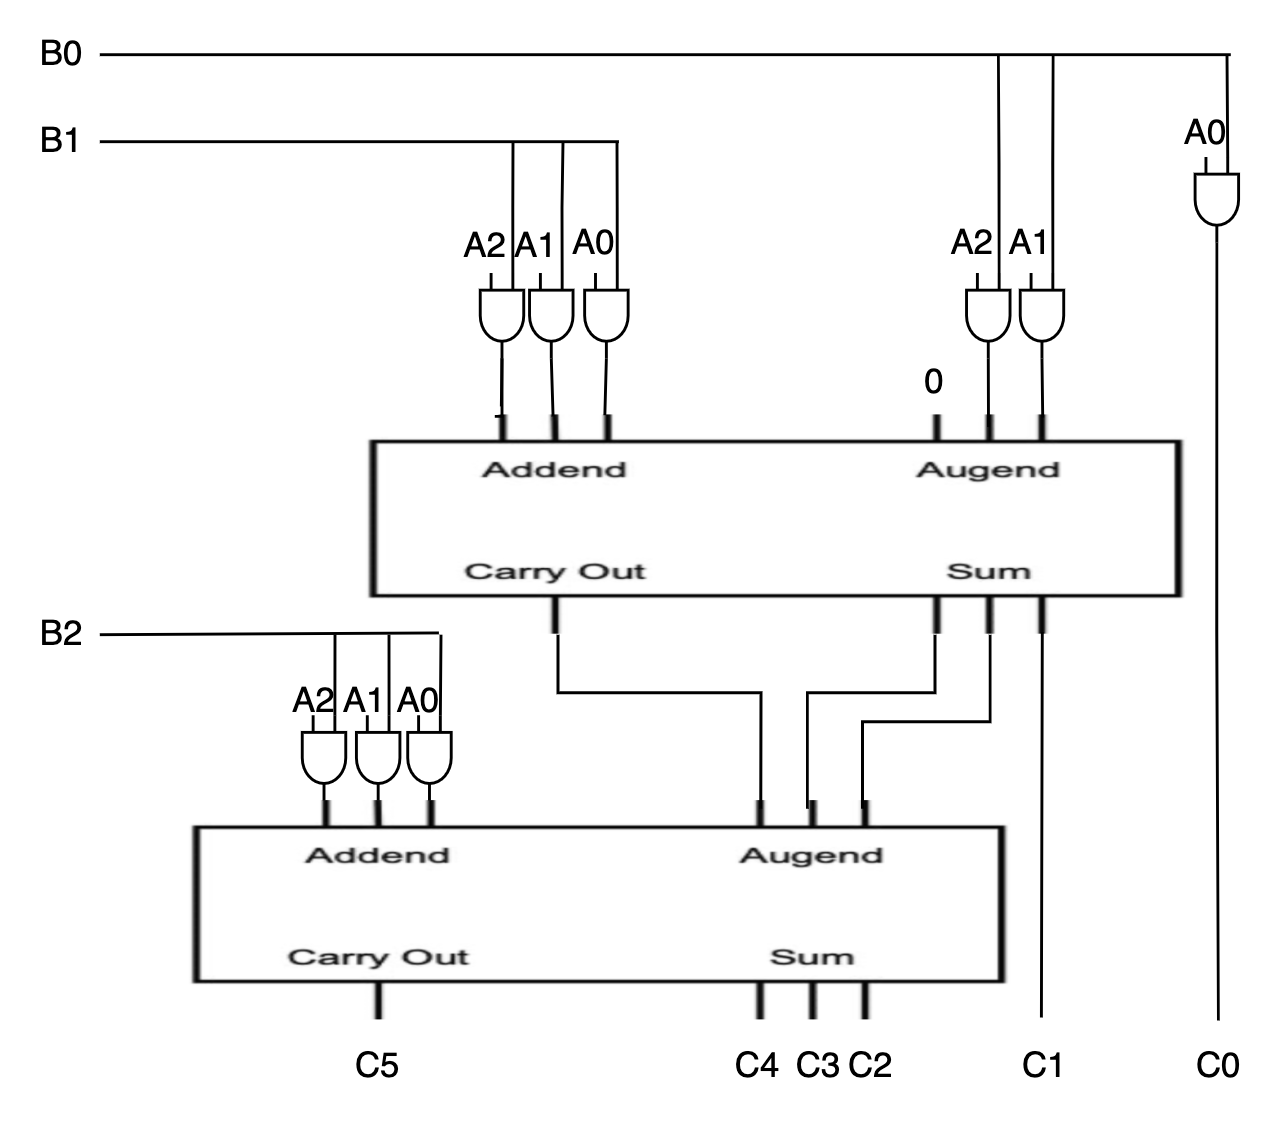
\includegraphics[width=0.5\textwidth]{fig/q4}}

\par The circuit can be represented as the following logic formulas:
\begin{align*}
C_0&=A_0B_0\\
C_1&=(A_1B_0)\oplus(A_0B_1)\\
C_2&=(A_2B_0)\oplus(A_1B_1)\oplus(A_0B_2)\oplus(A_1B_0A_0B_1)\\
C_3&=(A_2B_1)\oplus(A_1B_2)\oplus(A_2B_0A_1B_1A_0B_2B_0)\\
C_4&=(A_2B_2)\oplus(A_2B_0A_1B_1A_0B_2B_0)\\
C_5&=A_2B_0A_1B_1A_0B_2B_0
\end{align*}
\vspace{-2em}
